\section{Precision Model}

\subsection{Overview}

\frame{
    \frametitle{Loss of Precision with the Types Summary}
    \begin{columns}[c]
        \column{.6\textwidth}
        \begin{figure}
            \centering
            \resizebox{.9\textwidth}{!}{
                \begin{tikzpicture}[->,>=stealth',node distance=3.5cm]
    \node [draw,circle] (n0) {$v_0$};
    \node [draw,circle,above of = n0] (effi) {Effi\ldots};
    \node [red,draw,circle,right of = n0] (n2) {$v_1$};
    \node [draw,circle,below of = n2,yshift=-1cm] (n1) {$v_2$};
    \node [blue,draw,circle,right of = n2] (n3) {$v_3$};
    \node [draw,circle,right of = n3] (n6) {$v_6$};
    \node [draw,circle,below of = n6,yshift=-1cm] (n4) {$v_4$};
    \node [draw,circle,below of = n2,yshift=1.25cm] (person) {Person};
    \node [draw,circle,below of = n1] (ren) {Renaud};
    \node [draw,circle,above of = n2] (ste) {St\'ephane};
    \node [draw,circle,right of = n4] (n5) {$v_5$};
    \node [draw,circle,right of = n6] (n7) {$v_7$};
    \node [draw,circle,above right of = n4,xshift=-.7cm] (place) {Place};
    \node [draw,circle,above of = n7,yshift=0cm] (country) {Country};
    \node [draw,circle,below of = n4] (deri) {DERI};
    \node [draw,circle,below of = n5] (fbk) {FBK};
    \node [draw,circle,above left of = n3,xshift=1cm] (city) {City};
    \node [draw,circle,above right of = n3,xshift=-1cm] (gal) {Galway};
    \node [draw,circle,right of = n7] (rome) {Rome};
    \node [draw,circle,above of = n6] (ire) {Ireland};

    \path
        (n7) edge node[fill=white] {capital} (rome)
        (n6) edge node[fill=white] {label} (ire)

        (n3) edge node[fill=white] {label} (gal)
        (n3) edge node[fill=white] {type} (city)

        (n4) edge node[fill=white] {label} (deri)
        (n5) edge node[fill=white] {label} (fbk)

        (n6) edge node[fill=white] {type} (country)
        (n7) edge node[fill=white] {type} (country)

        (n4) edge node[fill=white] {type} (place)
        (n5) edge node[fill=white] {type} (place)
        (n6) edge node[fill=white] {type} (place)
        (n7) edge node[fill=white] {type} (place)

        (n3) edge node[fill=white] {location} (n6)
        (n4) edge node[fill=white] {location} (n6)
        (n5) edge node[fill=white] {location} (n7)
        (n1) edge node[fill=white] {name} (ren)
        (n2) edge node[fill=white] {name} (ste)
        (n1) edge node[fill=white] {type} (person)
        (n2) edge node[fill=white] {type} (person)
        (n0) edge node[fill=white] {title} (effi)
        (n0) edge[bend right] node[fill=white] {creator} (n2)
        (n0) edge[bend left] node[fill=white] {author} (n2)
        (n0) edge node[fill=white] {author} (n1)
        (n1) edge node[fill=white] {lives} (n3)
        (n1) edge node[fill=white] {works} (n4)
        (n2) edge node[fill=white] {lives} (n3)
        (n2) edge[near end] node[fill=white] {works} (n4)
    ;
\end{tikzpicture}
%% vim: et:sw=4

            }
            \caption{An entity graph describing people, places, and their relationships.}
        \end{figure}

        \column{.4\textwidth}
        \begin{figure}
            \centering
            \resizebox{.9\textwidth}{!}{
                \setbeamercovered{invisible}
\begin{tikzpicture}[->,>=stealth',node distance=4cm]
    \node [draw,circle] (h1) {$S_1$};
    \node [draw,circle,above right of = h1] (h2) {$S_2$};
    \node [draw,circle,below right of = h1] (h3) {$S_3$};
    \node [draw,circle,above right of = h3] (h4) {$S_4$};
    \node [draw,circle,above of = h1] (person) {Person};
    \node [draw,circle,above of = h2] (city) {City};
    \node [draw,circle,above of = h4] (country) {Country};
    \node [draw,circle,below right of = h4,xshift=-1cm] (place) {Place};
    \node [draw,circle,below of = h2,yshift=1cm] (c2) {$S_5$};

    \uncover<2-6>{
        \node [green highlight node,draw,circle] (h1) {$S_1$};
        \node [green highlight node,draw,circle,below right of = h1] (h3) {$S_3$};
        \draw [green highlight edge] (h1) edge[bend right] (h3);
    }
    \uncover<3-6>{
        \node [green highlight node,draw,circle,below right of = h1] (h3) {$S_3$};
        \node [green highlight node,draw,circle,above right of = h3] (h4) {$S_4$};
        \draw [green highlight edge] (h3) edge[bend right] (h4);
    }
    \uncover<4-6>{
        \node [green highlight node,draw,circle,above right of = h3] (h4) {$S_4$};
        \node [green highlight node,draw,circle,below of = h2,yshift=1cm] (c2) {$S_5$};
        \draw [green highlight edge] (h4) edge[bend left] (c2);
    }

    \path
        (h1) edge node[fill=white] {name} (c2)
        (h3) edge node[fill=white] {label} (c2)
        (h2) edge node[fill=white] {label} (c2)
        (h4) edge[bend right] node[fill=white] {label} (c2)
        (h4) edge[bend left] node[fill=white] {capital} (c2)

        (h1) edge node[fill=white] {type} (person)
        (h2) edge node[fill=white] {type} (city)
        (h4) edge node[near end,fill=white] {type} (country)
        (h4) edge node[fill=white] {type} (place)
        (h3) edge node[fill=white] {type} (place)
        (h1) edge[bend left] node[fill=white] {lives} (h2)
        (h1) edge[bend right] node[fill=white] {works} (h3)
        (h2) edge[bend left] node[fill=white] {location} (h4)
        (h3) edge[bend right] node[fill=white] {location} (h4)
        ;
\end{tikzpicture}
\setbeamercovered{transparent}
%% vim: et:sw=4

            }
            \caption{Types summary of the entity graph.}
        \end{figure}
    \end{columns}
}

\subsection{Model}

\frame{
    \frametitle{Ordering of Graph Summaries}
    \vspace{2em}
    \begin{block}{Partial Relation}
        \begin{figure}
            \centering
            \resizebox{.6\textwidth}{!}{
                \setbeamercovered{invisible}
\begin{tikzpicture}[->,>=stealth',node distance=3cm]
    \node (g) {$G$};
    \node[right of = g] (g1) {$\mathcal{S}_1$};
    \node[right of = g1] (g2) {$\mathcal{S}_2$};

    \uncover<2->{
        \draw[red] (g1) edge node[red,above] {$R_3$} (g2);
    }

    \path
        (g) edge node[above] {$R_1$} (g1)
        (g) edge [bend right=20] node[below] {$R_2$} (g2)
        ;
\end{tikzpicture}
\setbeamercovered{transparent}
%% vim: et:sw=4

            }
        \end{figure}
    \end{block}
    \vspace{-2em}
    \uncover<3->{
        \begin{block}{Graph Lattice}
            \begin{figure}
                \centering
                \resizebox{.8\textwidth}{!}{
                    \begin{tikzpicture}[->,>=stealth',node distance=2cm]
\node (base) {\emph{Infimum}};
\node[right of = base] (ioat) {$R_{ioat}$};
\node[right of = ioat] (ta1) {$R_{iat}$};
\node[above of = ta1] (at) {$R_{at}$};
\node[below of = ta1] (ioa) {$R_{ioa}$};
\node[right of = at] (t) {$R_t$};
\node[right of = ta1] (a) {$R_a$};
\node[right of = ioa] (a1) {$R_{ia}$};
\node[right of = t] (st) {$R_{ut}$};
\node[right of = a] (phantom) {};
\node[right of = phantom] (apex) {\emph{Supremum}};

\path
(base) edge (ioat)
(ioat) edge (ta1)
(ioat) edge (at)
(ioat) edge (ioa)
(at) edge (t)
(at) edge (a)
(ioa) edge (a)
(ioa) edge (a1)
(ta1) edge (t)
(ta1) edge (a1)
(t) edge (st)
(st) edge (apex)
(a) edge (apex)
(a1) edge (apex)
;
\end{tikzpicture}
%% vim: et:sw=4

                }
            \end{figure}
        \end{block}
    }
}

\frame{
    \frametitle{Model}
    \begin{block}{Comparison}
        \begin{itemize}
            \item Leverage the partial relation for ordering the summaries
            \item Compare a summary against the original graph
            \item Compute how many errors the summarisation committed
        \end{itemize}
    \end{block}
}

\frame{
    \frametitle{An Example:\\Evaluation of the Summary Precision}
    \begin{columns}[c]
        \column{.6\textwidth}
        \begin{figure}
            \centering
            \resizebox{.9\textwidth}{!}{
                \setbeamercovered{invisible}
\begin{tikzpicture}[->,>=stealth',node distance=3.5cm]
    \uncover<1-1>{
        \node [draw,circle] (n2) {$v_1$};
        \node [draw,circle,below of = n2,yshift=-1cm] (n1) {$v_2$};
        \node [draw,circle,right of = n2] (n3) {$v_3$};
        \node [draw,circle,right of = n3] (n6) {$v_6$};
        \node [draw,circle,below of = n6,yshift=-1cm] (n4) {$v_4$};
        \node [draw,circle,below of = n2,yshift=1.25cm] (person) {Person};
        \node [draw,circle,below of = n1] (ren) {Renaud};
        \node [draw,circle,above of = n2] (ste) {St\'ephane};
        \node [draw,circle,right of = n4] (n5) {$v_5$};
        \node [draw,circle,right of = n6] (n7) {$v_7$};
        \node [draw,circle,above right of = n4,xshift=-.7cm] (place) {Place};
        \node [draw,circle,above of = n7,yshift=0cm] (country) {Country};
        \node [draw,circle,below of = n4] (deri) {DERI};
        \node [draw,circle,below of = n5] (fbk) {FBK};
        \node [draw,circle,above left of = n3,xshift=1cm] (city) {City};
        \node [draw,circle,above right of = n3,xshift=-1cm] (gal) {Galway};
        \node [draw,circle,above right of = n7] (rome) {Rome};
        \node [draw,circle,above of = n6] (ire) {Ireland};

        \path
            (n7) edge node[fill=white] {capital} (rome)
            (n6) edge node[fill=white] {label} (ire)
    
            (n3) edge node[fill=white] {label} (gal)
            (n3) edge node[fill=white] {type} (city)
    
            (n4) edge node[fill=white] {label} (deri)
            (n5) edge node[fill=white] {label} (fbk)
    
            (n6) edge node[fill=white] {type} (country)
            (n7) edge node[fill=white] {type} (country)
    
            (n4) edge node[fill=white] {type} (place)
            (n5) edge node[fill=white] {type} (place)
            (n6) edge node[fill=white] {type} (place)
            (n7) edge node[fill=white] {type} (place)
    
            (n3) edge node[fill=white] {location} (n6)
            (n4) edge node[fill=white] {location} (n6)
            (n5) edge node[fill=white] {location} (n7)
            (n1) edge node[fill=white] {name} (ren)
            (n2) edge node[fill=white] {name} (ste)
            (n1) edge node[fill=white] {type} (person)
            (n2) edge node[fill=white] {type} (person)
            (n1) edge node[fill=white] {lives} (n3)
            (n1) edge node[fill=white] {works} (n4)
            (n2) edge node[fill=white] {lives} (n3)
            (n2) edge[near end] node[fill=white] {works} (n4)
        ;
    }

    \uncover<2->{
        \node [draw,circle] (n2) {7};
        \node [draw,circle,below of = n2,yshift=-1cm] (n1) {13};
        \node [draw,circle,right of = n2] (n3) {8};
        \node [draw,circle,right of = n3] (n6) {9};
        \node [draw,circle,below of = n6,yshift=-1cm] (n4) {14};
        \node [draw,circle,below of = n2,yshift=1.25cm] (person) {11};
        \node [draw,circle,below of = n1] (ren) {16};
        \node [draw,circle,above of = n2] (ste) {1};
        \node [draw,circle,right of = n4] (n5) {15};
        \node [draw,circle,right of = n6] (n7) {10};
        \node [draw,circle,above right of = n4,xshift=-.7cm] (place) {12};
        \node [draw,circle,above of = n7,yshift=0cm] (country) {5};
        \node [draw,circle,below of = n4] (deri) {17};
        \node [draw,circle,below of = n5] (fbk) {18};
        \node [draw,circle,above left of = n3,xshift=1cm] (city) {2};
        \node [draw,circle,above right of = n3,xshift=-1cm] (gal) {3};
        \node [draw,circle,above right of = n7] (rome) {6};
        \node [draw,circle,above of = n6] (ire) {4};

        \path
            (n7) edge node[fill=white] {capital} (rome)
            (n6) edge node[fill=white] {label} (ire)
    
            (n3) edge node[fill=white] {label} (gal)
            (n3) edge node[fill=white] {type} (city)
    
            (n4) edge node[fill=white] {label} (deri)
            (n5) edge node[fill=white] {label} (fbk)
    
            (n6) edge node[fill=white] {type} (country)
            (n7) edge node[fill=white] {type} (country)
    
            (n4) edge node[fill=white] {type} (place)
            (n5) edge node[fill=white] {type} (place)
            (n6) edge node[fill=white] {type} (place)
            (n7) edge node[fill=white] {type} (place)
    
            (n3) edge node[fill=white] {location} (n6)
            (n4) edge node[fill=white] {location} (n6)
            (n5) edge node[fill=white] {location} (n7)
            (n1) edge node[fill=white] {name} (ren)
            (n2) edge node[fill=white] {name} (ste)
            (n1) edge node[fill=white] {type} (person)
            (n2) edge node[fill=white] {type} (person)
            (n1) edge node[fill=white] {lives} (n3)
            (n1) edge node[fill=white] {works} (n4)
            (n2) edge node[fill=white] {lives} (n3)
            (n2) edge[near end] node[fill=white] {works} (n4)
        ;
    }
\end{tikzpicture}
\setbeamercovered{transparent}
%% vim: et:sw=4

            }
        \end{figure}

        \column{.4\textwidth}
        \begin{figure}
            \centering
            \resizebox{.9\textwidth}{!}{
                \setbeamercovered{invisible}
\begin{tikzpicture}[->,>=stealth',node distance=4cm]
    \uncover<1-1>{
        \node [draw,circle] (h1) {$S_1$};
        \node [draw,circle,above right of = h1] (h2) {$S_2$};
        \node [draw,circle,below right of = h1] (h3) {$S_3$};
        \node [draw,circle,above right of = h3] (h4) {$S_4$};
        \node [draw,circle,above of = h1] (person) {Person};
        \node [draw,circle,above of = h2] (city) {City};
        \node [draw,circle,above of = h4] (country) {Country};
        \node [draw,circle,below right of = h4,xshift=-1cm] (place) {Place};
        \node [draw,circle,below of = h2,yshift=1cm] (c2) {$S_5$};

        \path
            (h1) edge node[fill=white] {name} (c2)
            (h3) edge node[fill=white] {label} (c2)
            (h2) edge node[fill=white] {label} (c2)
            (h4) edge[bend right] node[fill=white] {label} (c2)
            (h4) edge[bend left] node[fill=white] {capital} (c2)
    
            (h1) edge node[fill=white] {type} (person)
            (h2) edge node[fill=white] {type} (city)
            (h4) edge node[near end,fill=white] {type} (country)
            (h4) edge node[fill=white] {type} (place)
            (h3) edge node[fill=white] {type} (place)
            (h1) edge[bend left] node[fill=white] {lives} (h2)
            (h1) edge[bend right] node[fill=white] {works} (h3)
            (h2) edge[bend left] node[fill=white] {location} (h4)
            (h3) edge[bend right] node[fill=white] {location} (h4)
            ;
    }

    \uncover<2->{
        \node [draw,circle] (h1) {E};
        \node [draw,circle,above right of = h1] (h2) {D};
        \node [draw,circle,below right of = h1] (h3) {H};
        \node [draw,circle,above right of = h3] (h4) {G};
        \node [draw,circle,above of = h1] (person) {A};
        \node [draw,circle,above of = h2] (city) {B};
        \node [draw,circle,above of = h4] (country) {C};
        \node [draw,circle,below right of = h4,xshift=-1cm] (place) {I};
        \node [draw,circle,below of = h2,yshift=1cm] (c2) {F};

        \path
            (h1) edge node[fill=white] {name} (c2)
            (h3) edge node[fill=white] {label} (c2)
            (h2) edge node[fill=white] {label} (c2)
            (h4) edge[bend right] node[fill=white] {label} (c2)
            (h4) edge[bend left] node[fill=white] {capital} (c2)
    
            (h1) edge node[fill=white] {type} (person)
            (h2) edge node[fill=white] {type} (city)
            (h4) edge node[near end,fill=white] {type} (country)
            (h4) edge node[fill=white] {type} (place)
            (h3) edge node[fill=white] {type} (place)
            (h1) edge[bend left] node[fill=white] {lives} (h2)
            (h1) edge[bend right] node[fill=white] {works} (h3)
            (h2) edge[bend left] node[fill=white] {location} (h4)
            (h3) edge[bend right] node[fill=white] {location} (h4)
            ;
    }
\end{tikzpicture}
\setbeamercovered{transparent}
%% vim: et:sw=4

            }
        \end{figure}
    \end{columns}
}

\frame{
    \frametitle{An Example:\\Evaluation of the Summary Precision}
    \resizebox{\textwidth}{!}{
        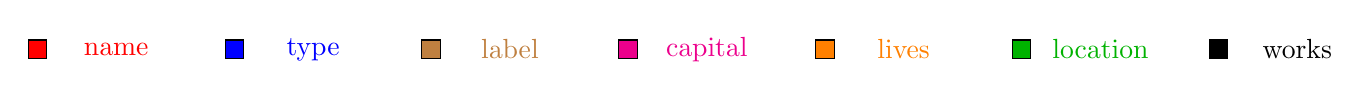
\begin{tikzpicture}[]
    \node[font=\bfseries,draw,fill=red] (nameColor) {};
    \node[red,right of = nameColor] (name) {name};

    \node[font=\bfseries,draw,fill=blue,right of = name,xshift=.5cm] (typeColor) {};
    \node[blue,right of = typeColor] (type) {type};

    \node[font=\bfseries,draw,fill=brown,right of = type,xshift=.5cm] (labelColor) {};
    \node[brown,right of = labelColor] (label) {label};

    \node[font=\bfseries,draw,fill=magenta,right of = label,xshift=.5cm] (capitalColor) {};
    \node[magenta,right of = capitalColor] (capital) {capital};

    \node[font=\bfseries,draw,fill=orange,right of = capital,xshift=.5cm] (livesColor) {};
    \node[orange,right of = livesColor] (lives) {lives};

    \node[font=\bfseries,draw,fill=black!30!green,right of = lives,xshift=.5cm] (locationColor) {};
    \node[black!30!green,right of = locationColor] (location) {location};

    \node[font=\bfseries,draw,fill=black,right of = location,xshift=.5cm] (worksColor) {};
    \node[black,right of = worksColor] (works) {works};
\end{tikzpicture}
%% vim: et:sw=4

    }
    \vspace{.25em}
    \begin{columns}[c]
        \column{.5\textwidth}
        \resizebox{\textwidth}{!}{
            \pgfplotstableread[header=false]{graph-matrix.dat}{\graph} 
\pgfplotstablegetrowsof{graph-matrix.dat}
\pgfmathsetmacro{\rows}{\pgfplotsretval}

%name = 1 = red
%type = 2 = blue
%label = 3 = brown
%capital = 4 = magenta
%lives = 5 = orange
%location = 6 = black!30!green
%works = 7 = black

\begin{tikzpicture}[draw=black, ultra thick]
    \foreach \col in {0,...,\rows} {%
        \foreach \row in {0,...,\rows} {%
            \ifthenelse{\row=0 \AND \col=0}{
                \node [Square] at ($(\col,-\row)-(0.5,0.5)$) {};
            }
            {
                \ifthenelse{\row=0}{
                    \node [Square] at ($(\col,-\row)-(0.5,0.5)$) {\col};
                }
                {
                    \ifthenelse{\col=0}{
                        \node [Square] at ($(\col,-\row)-(0.5,0.5)$) {\row};
                    }
                    {
                        \pgfmathsetmacro{\x}{int(\row-1)}
                        \pgfmathsetmacro{\y}{int(\col-1)}

                        \pgfplotstablegetelem{\x}{\y}\of{\graph} 

                        \begin{switch}{\pgfplotsretval}
                            \case{0}{
                                \node [Square] at ($(\col,-\row)-(0.5,0.5)$) {};
                            }
                            \case{1}{
                                \node [Red Square] at ($(\col,-\row)-(0.5,0.5)$) {};
                            }
                            \case{2}{
                                \node [Blue Square] at ($(\col,-\row)-(0.5,0.5)$) {};
                            }
                            \case{3}{
                                \node [Brown Square] at ($(\col,-\row)-(0.5,0.5)$) {};
                            }
                            \case{4}{
                                \node [Magenta Square] at ($(\col,-\row)-(0.5,0.5)$) {};
                            }
                            \case{5}{
                                \node [Orange Square] at ($(\col,-\row)-(0.5,0.5)$) {};
                            }
                            \case{6}{
                                \node [Green Square] at ($(\col,-\row)-(0.5,0.5)$) {};
                            }
                            \case{7}{
                                \node [Black Square] at ($(\col,-\row)-(0.5,0.5)$) {};
                            }
                        \end{switch}
                    }
                }
            }
        }
    }
\end{tikzpicture}
%% vim: et:sw=4

        }

        \column{.55\textwidth}
        \resizebox{\textwidth}{!}{
            \pgfplotstableread[header=false]{images/precision/classes-matrix.dat}{\classes} 
\pgfplotstablegetrowsof{images/precision/classes-matrix.dat}
\pgfmathsetmacro{\classesRows}{\pgfplotsretval}

%%%
%%% numbers mapping in the matrix
%%%

%name = 1 = red
%type = 2 = blue
%label = 3 = brown
%capital = 4 = magenta
%lives = 5 = orange
%location = 6 = black!30!green
%works = 7 = black

%label + capital = 8

%%%
%%% how many nodes per summnode
%%%

%A = 1
%B = 1
%C = 1
%D = 1
%E = 2
%F = 7
%G = 2
%H = 2
%I = 1

\begin{tikzpicture}[draw=black, ultra thick]
    \foreach \col in {0,...,\classesRows} {%
        \foreach \row in {0,...,\classesRows} {%
            \ifthenelse{\row=0 \AND \col=0}{
                \node [Square] at ($(\col,-\row)-(0.5,0.5)$) {};
            }
            {
                \ifthenelse{\row=0}{
                    \begin{switch}{\col}
                        \case{1}{
                            \node [Square] at ($(\col,-\row)-(0.5,0.5)$) {A};
                        }
                        \case{2}{
                            \node [Square] at ($(\col,-\row)-(0.5,0.5)$) {B};
                        }
                        \case{3}{
                            \node [Square] at ($(\col,-\row)-(0.5,0.5)$) {C};
                        }
                        \case{4}{
                            \node [Square] at ($(\col,-\row)-(0.5,0.5)$) {D};
                        }
                        \case{5}{
                            \node [Square] at ($(\col,-\row)-(0.5,0.5)$) {E};
                        }
                        \case{6}{
                            \node [Square] at ($(\col,-\row)-(0.5,0.5)$) {F};
                        }
                        \case{7}{
                            \node [Square] at ($(\col,-\row)-(0.5,0.5)$) {G};
                        }
                        \case{8}{
                            \node [Square] at ($(\col,-\row)-(0.5,0.5)$) {H};
                        }
                        \case{9}{
                            \node [Square] at ($(\col,-\row)-(0.5,0.5)$) {I};
                        }
                    \end{switch}
                }
                {
                    \ifthenelse{\col=0}{
                        \begin{switch}{\row}
                            \case{1}{
                                \node [Square] at ($(\col,-\row)-(0.5,0.5)$) {A};
                            }
                            \case{2}{
                                \node [Square] at ($(\col,-\row)-(0.5,0.5)$) {B};
                            }
                            \case{3}{
                                \node [Square] at ($(\col,-\row)-(0.5,0.5)$) {C};
                            }
                            \case{4}{
                                \node [Square] at ($(\col,-\row)-(0.5,0.5)$) {D};
                            }
                            \case{5}{
                                \node [Square] at ($(\col,-\row)-(0.5,0.5)$) {E};
                            }
                            \case{6}{
                                \node [Square] at ($(\col,-\row)-(0.5,0.5)$) {F};
                            }
                            \case{7}{
                                \node [Square] at ($(\col,-\row)-(0.5,0.5)$) {G};
                            }
                            \case{8}{
                                \node [Square] at ($(\col,-\row)-(0.5,0.5)$) {H};
                            }
                            \case{9}{
                                \node [Square] at ($(\col,-\row)-(0.5,0.5)$) {I};
                            }
                        \end{switch}
                    }
                    {
                        \pgfmathsetmacro{\x}{int(\row-1)}
                        \pgfmathsetmacro{\y}{int(\col-1)}

                        \pgfplotstablegetelem{\x}{\y}\of{\classes} 

                        \begin{switch}{\pgfplotsretval}
                            \case{0}{
                                \node [Square] at ($(\col,-\row)-(0.5,0.5)$) {};
                            }
                            \case{1}{
                                \node [Red Square] at ($(\col,-\row)-(0.5,0.5)$) {};
                            }
                            \case{2}{
                                \node [Blue Square] at ($(\col,-\row)-(0.5,0.5)$) {};
                            }
                            \case{3}{
                                \node [Brown Square] at ($(\col,-\row)-(0.5,0.5)$) {};
                            }
                            \case{4}{
                                \node [Magenta Square] at ($(\col,-\row)-(0.5,0.5)$) {};
                            }
                            \case{5}{
                                \node [Orange Square] at ($(\col,-\row)-(0.5,0.5)$) {};
                            }
                            \case{6}{
                                \node [Green Square] at ($(\col,-\row)-(0.5,0.5)$) {};
                            }
                            \case{7}{
                                \node [Black Square] at ($(\col,-\row)-(0.5,0.5)$) {};
                            }
                            \case{8}{
                                %% two colors: magenta and brown. Magenta is drown with stripes below
                                \node [Magenta Square] at ($(\col,-\row)-(0.5,0.5)$) {};
                                \begin{scope}
                                    \clip (\col-1+.027,-\row-.027) rectangle (\col-.027,-\row-1+.027);
                                    \foreach \x in {0,0.4,...,\classesRows} {%
                                        \draw [brown,line width=4pt] (0,\x) -- (\classesRows,\x - \classesRows);
                                        \draw [brown,line width=4pt] (0,-\x) -- (\classesRows,-\x - \classesRows);
                                    }
                                \end{scope}
                            }
                        \end{switch}
                    }
                }
            }
        }
    }
\end{tikzpicture}
%% vim: et:sw=4

        }
    \end{columns}
}

\frame{
    \frametitle{An Example:\\Evaluation of the Summary Precision}
    \resizebox{\textwidth}{!}{
        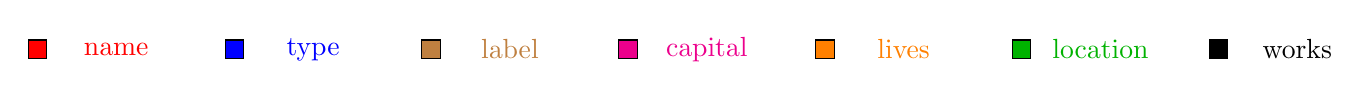
\begin{tikzpicture}[]
    \node[font=\bfseries,draw,fill=red] (nameColor) {};
    \node[red,right of = nameColor] (name) {name};

    \node[font=\bfseries,draw,fill=blue,right of = name,xshift=.5cm] (typeColor) {};
    \node[blue,right of = typeColor] (type) {type};

    \node[font=\bfseries,draw,fill=brown,right of = type,xshift=.5cm] (labelColor) {};
    \node[brown,right of = labelColor] (label) {label};

    \node[font=\bfseries,draw,fill=magenta,right of = label,xshift=.5cm] (capitalColor) {};
    \node[magenta,right of = capitalColor] (capital) {capital};

    \node[font=\bfseries,draw,fill=orange,right of = capital,xshift=.5cm] (livesColor) {};
    \node[orange,right of = livesColor] (lives) {lives};

    \node[font=\bfseries,draw,fill=black!30!green,right of = lives,xshift=.5cm] (locationColor) {};
    \node[black!30!green,right of = locationColor] (location) {location};

    \node[font=\bfseries,draw,fill=black,right of = location,xshift=.5cm] (worksColor) {};
    \node[black,right of = worksColor] (works) {works};
\end{tikzpicture}
%% vim: et:sw=4

    }
    \vspace{.25em}
    \begin{columns}[c]
        \column{.5\textwidth}
        \resizebox{\textwidth}{!}{
            \pgfplotstableread[header=false]{graph-matrix.dat}{\graph} 
\pgfplotstablegetrowsof{graph-matrix.dat}
\pgfmathsetmacro{\rows}{\pgfplotsretval}

%name = 1 = red
%type = 2 = blue
%label = 3 = brown
%capital = 4 = magenta
%lives = 5 = orange
%location = 6 = black!30!green
%works = 7 = black

\begin{tikzpicture}[draw=black, ultra thick]
    \foreach \col in {0,...,\rows} {%
        \foreach \row in {0,...,\rows} {%
            \ifthenelse{\row=0 \AND \col=0}{
                \node [Square] at ($(\col,-\row)-(0.5,0.5)$) {};
            }
            {
                \ifthenelse{\row=0}{
                    \node [Square] at ($(\col,-\row)-(0.5,0.5)$) {\col};
                }
                {
                    \ifthenelse{\col=0}{
                        \node [Square] at ($(\col,-\row)-(0.5,0.5)$) {\row};
                    }
                    {
                        \pgfmathsetmacro{\x}{int(\row-1)}
                        \pgfmathsetmacro{\y}{int(\col-1)}

                        \pgfplotstablegetelem{\x}{\y}\of{\graph} 

                        \begin{switch}{\pgfplotsretval}
                            \case{0}{
                                \node [Square] at ($(\col,-\row)-(0.5,0.5)$) {};
                            }
                            \case{1}{
                                \node [Red Square] at ($(\col,-\row)-(0.5,0.5)$) {};
                            }
                            \case{2}{
                                \node [Blue Square] at ($(\col,-\row)-(0.5,0.5)$) {};
                            }
                            \case{3}{
                                \node [Brown Square] at ($(\col,-\row)-(0.5,0.5)$) {};
                            }
                            \case{4}{
                                \node [Magenta Square] at ($(\col,-\row)-(0.5,0.5)$) {};
                            }
                            \case{5}{
                                \node [Orange Square] at ($(\col,-\row)-(0.5,0.5)$) {};
                            }
                            \case{6}{
                                \node [Green Square] at ($(\col,-\row)-(0.5,0.5)$) {};
                            }
                            \case{7}{
                                \node [Black Square] at ($(\col,-\row)-(0.5,0.5)$) {};
                            }
                        \end{switch}
                    }
                }
            }
        }
    }
\end{tikzpicture}
%% vim: et:sw=4

        }

        \column{.5\textwidth}
        \resizebox{\textwidth}{!}{
            \pgfplotstableread[header=false]{images/precision/inferred-graph-matrix.dat}{\classes} 
\pgfplotstablegetrowsof{images/precision/inferred-graph-matrix.dat}
\pgfmathsetmacro{\classesRows}{\pgfplotsretval}

%%%
%%% numbers mapping in the matrix
%%%

%name = 1 = red
%type = 2 = blue
%label = 3 = brown
%capital = 4 = magenta
%lives = 5 = orange
%location = 6 = black!30!green
%works = 7 = black

%label + capital = 8

%%%
%%% how many nodes per summnode
%%%

%A = 1
%B = 1
%C = 1
%D = 1
%E = 2
%F = 7
%G = 2
%H = 2
%I = 1

\begin{tikzpicture}[draw=black, ultra thick]
    \foreach \col in {0,...,\classesRows} {%
        \foreach \row in {0,...,\classesRows} {%
            \ifthenelse{\row=0}{
                \begin{switch}{\col}
                    \case{1}{ % A - person - 11
                        \node [Square] at ($(\col,-\row)-(0.5,0.5)$) {11};
                    }
                    \case{2}{ % B - city - 2
                        \node [Square] at ($(\col,-\row)-(0.5,0.5)$) {2};
                    }
                    \case{3}{ % C - country - 5
                        \node [Square] at ($(\col,-\row)-(0.5,0.5)$) {5};
                    }
                    \case{4}{ % D - v3 - 8
                        \node [Square] at ($(\col,-\row)-(0.5,0.5)$) {8};
                    }
                    \case{5}{ % E - v1 - 7
                        \node [Square] at ($(\col,-\row)-(0.5,0.5)$) {7};
                    }
                    \case{6}{ % E - v2 - 13
                        \node [Square] at ($(\col,-\row)-(0.5,0.5)$) {13};
                    }
                    \case{7}{ % F - stephane - 1
                        \node [Square] at ($(\col,-\row)-(0.5,0.5)$) {1};
                    }
                    \case{8}{ % F - galway - 3
                        \node [Square] at ($(\col,-\row)-(0.5,0.5)$) {3};
                    }
                    \case{9}{ % F - ireland - 4
                        \node [Square] at ($(\col,-\row)-(0.5,0.5)$) {4};
                    }
                    \case{10}{ % F - rome - 6
                        \node [Square] at ($(\col,-\row)-(0.5,0.5)$) {6};
                    }
                    \case{11}{ % F - renaud - 16
                        \node [Square] at ($(\col,-\row)-(0.5,0.5)$) {16};
                    }
                    \case{12}{ % F - deri - 17
                        \node [Square] at ($(\col,-\row)-(0.5,0.5)$) {17};
                    }
                    \case{13}{ % F - fbk - 18
                        \node [Square] at ($(\col,-\row)-(0.5,0.5)$) {18};
                    }
                    \case{14}{ % G - v6 - 9
                        \node [Square] at ($(\col,-\row)-(0.5,0.5)$) {9};
                    }
                    \case{15}{ % G - v7 - 10
                        \node [Square] at ($(\col,-\row)-(0.5,0.5)$) {10};
                    }
                    \case{16}{ % H - v4 - 14
                        \node [Square] at ($(\col,-\row)-(0.5,0.5)$) {14};
                    }
                    \case{17}{ % H - v5 - 15
                        \node [Square] at ($(\col,-\row)-(0.5,0.5)$) {15};
                    }
                    \case{18}{ % I - place - 12
                        \node [Square] at ($(\col,-\row)-(0.5,0.5)$) {12};
                    }
                \end{switch}
            }
            {
                \ifthenelse{\col=0}{
                    \begin{switch}{\row}
                        \case{1}{ % A - person - 11
                            \node [Square] at ($(\col,-\row)-(0.5,0.5)$) {11};
                        }
                        \case{2}{ % B - city - 2
                            \node [Square] at ($(\col,-\row)-(0.5,0.5)$) {2};
                        }
                        \case{3}{ % C - country - 5
                            \node [Square] at ($(\col,-\row)-(0.5,0.5)$) {5};
                        }
                        \case{4}{ % D - v3 - 8
                            \node [Square] at ($(\col,-\row)-(0.5,0.5)$) {8};
                        }
                        \case{5}{ % E - v1 - 7
                            \node [Square] at ($(\col,-\row)-(0.5,0.5)$) {7};
                        }
                        \case{6}{ % E - v2 - 13
                            \node [Square] at ($(\col,-\row)-(0.5,0.5)$) {13};
                        }
                        \case{7}{ % F - stephane - 1
                            \node [Square] at ($(\col,-\row)-(0.5,0.5)$) {1};
                        }
                        \case{8}{ % F - galway - 3
                            \node [Square] at ($(\col,-\row)-(0.5,0.5)$) {3};
                        }
                        \case{9}{ % F - ireland - 4
                            \node [Square] at ($(\col,-\row)-(0.5,0.5)$) {4};
                        }
                        \case{10}{ % F - rome - 6
                            \node [Square] at ($(\col,-\row)-(0.5,0.5)$) {6};
                        }
                        \case{11}{ % F - renaud - 16
                            \node [Square] at ($(\col,-\row)-(0.5,0.5)$) {16};
                        }
                        \case{12}{ % F - deri - 17
                            \node [Square] at ($(\col,-\row)-(0.5,0.5)$) {17};
                        }
                        \case{13}{ % F - fbk - 18
                            \node [Square] at ($(\col,-\row)-(0.5,0.5)$) {18};
                        }
                        \case{14}{ % G - v6 - 9
                            \node [Square] at ($(\col,-\row)-(0.5,0.5)$) {9};
                        }
                        \case{15}{ % G - v7 - 10
                            \node [Square] at ($(\col,-\row)-(0.5,0.5)$) {10};
                        }
                        \case{16}{ % H - v4 - 14
                            \node [Square] at ($(\col,-\row)-(0.5,0.5)$) {14};
                        }
                        \case{17}{ % H - v5 - 15
                            \node [Square] at ($(\col,-\row)-(0.5,0.5)$) {15};
                        }
                        \case{18}{ % I - place - 12
                            \node [Square] at ($(\col,-\row)-(0.5,0.5)$) {12};
                        }
                    \end{switch}
                }
                {
                    \pgfmathsetmacro{\x}{int(\row-1)}
                    \pgfmathsetmacro{\y}{int(\col-1)}

                    \pgfplotstablegetelem{\x}{\y}\of{\classes} 

                    \begin{switch}{\pgfplotsretval}
                        \case{0}{
                            \node [Square] at ($(\col,-\row)-(0.5,0.5)$) {};
                        }
                        \case{1}{
                            \node [Red Square] at ($(\col,-\row)-(0.5,0.5)$) {};
                        }
                        \case{2}{
                            \node [Blue Square] at ($(\col,-\row)-(0.5,0.5)$) {};
                        }
                        \case{3}{
                            \node [Brown Square] at ($(\col,-\row)-(0.5,0.5)$) {};
                        }
                        \case{4}{
                            \node [Magenta Square] at ($(\col,-\row)-(0.5,0.5)$) {};
                        }
                        \case{5}{
                            \node [Orange Square] at ($(\col,-\row)-(0.5,0.5)$) {};
                        }
                        \case{6}{
                            \node [Green Square] at ($(\col,-\row)-(0.5,0.5)$) {};
                        }
                        \case{7}{
                            \node [Black Square] at ($(\col,-\row)-(0.5,0.5)$) {};
                        }
                        \case{8}{
                            %% two colors: magenta and brown. Magenta is drown with stripes below
                            \node [Magenta Square] at ($(\col,-\row)-(0.5,0.5)$) {};
                            \begin{scope}
                                \clip (\col-1+.027,-\row-.027) rectangle (\col-.027,-\row-1+.027);
                                \foreach \x in {0,0.4,...,\classesRows} {%
                                    \draw [brown,line width=4pt] (0,\x) -- (\classesRows,\x - \classesRows);
                                    \draw [brown,line width=4pt] (0,-\x) -- (\classesRows,-\x - \classesRows);
                                }
                            \end{scope}
                        }
                    \end{switch}
                }
            }
        }
    }
\end{tikzpicture}
%% vim: et:sw=4

        }
    \end{columns}
}

\frame{
    \frametitle{An Example:\\Evaluation of the Summary Precision}
    \resizebox{\textwidth}{!}{
        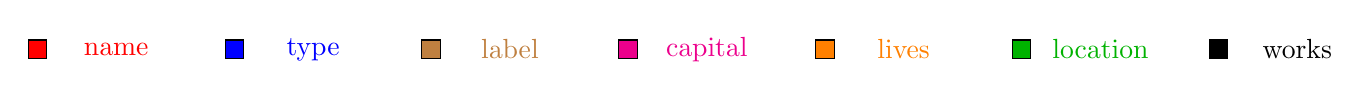
\begin{tikzpicture}[]
    \node[font=\bfseries,draw,fill=red] (nameColor) {};
    \node[red,right of = nameColor] (name) {name};

    \node[font=\bfseries,draw,fill=blue,right of = name,xshift=.5cm] (typeColor) {};
    \node[blue,right of = typeColor] (type) {type};

    \node[font=\bfseries,draw,fill=brown,right of = type,xshift=.5cm] (labelColor) {};
    \node[brown,right of = labelColor] (label) {label};

    \node[font=\bfseries,draw,fill=magenta,right of = label,xshift=.5cm] (capitalColor) {};
    \node[magenta,right of = capitalColor] (capital) {capital};

    \node[font=\bfseries,draw,fill=orange,right of = capital,xshift=.5cm] (livesColor) {};
    \node[orange,right of = livesColor] (lives) {lives};

    \node[font=\bfseries,draw,fill=black!30!green,right of = lives,xshift=.5cm] (locationColor) {};
    \node[black!30!green,right of = locationColor] (location) {location};

    \node[font=\bfseries,draw,fill=black,right of = location,xshift=.5cm] (worksColor) {};
    \node[black,right of = worksColor] (works) {works};
\end{tikzpicture}
%% vim: et:sw=4

    }
    \vspace{.25em}
    \begin{columns}[c]
        \column{.5\textwidth}
        \resizebox{\textwidth}{!}{
            \pgfplotstableread[header=false]{graph-matrix.dat}{\graph} 
\pgfplotstablegetrowsof{graph-matrix.dat}
\pgfmathsetmacro{\rows}{\pgfplotsretval}

%name = 1 = red
%type = 2 = blue
%label = 3 = brown
%capital = 4 = magenta
%lives = 5 = orange
%location = 6 = black!30!green
%works = 7 = black

\begin{tikzpicture}[draw=black, ultra thick]
    \foreach \col in {0,...,\rows} {%
        \foreach \row in {0,...,\rows} {%
            \ifthenelse{\row=0 \AND \col=0}{
                \node [Square] at ($(\col,-\row)-(0.5,0.5)$) {};
            }
            {
                \ifthenelse{\row=0}{
                    \node [Square] at ($(\col,-\row)-(0.5,0.5)$) {\col};
                }
                {
                    \ifthenelse{\col=0}{
                        \node [Square] at ($(\col,-\row)-(0.5,0.5)$) {\row};
                    }
                    {
                        \pgfmathsetmacro{\x}{int(\row-1)}
                        \pgfmathsetmacro{\y}{int(\col-1)}

                        \pgfplotstablegetelem{\x}{\y}\of{\graph} 

                        \begin{switch}{\pgfplotsretval}
                            \case{0}{
                                \node [Square] at ($(\col,-\row)-(0.5,0.5)$) {};
                            }
                            \case{1}{
                                \node [Red Square] at ($(\col,-\row)-(0.5,0.5)$) {};
                            }
                            \case{2}{
                                \node [Blue Square] at ($(\col,-\row)-(0.5,0.5)$) {};
                            }
                            \case{3}{
                                \node [Brown Square] at ($(\col,-\row)-(0.5,0.5)$) {};
                            }
                            \case{4}{
                                \node [Magenta Square] at ($(\col,-\row)-(0.5,0.5)$) {};
                            }
                            \case{5}{
                                \node [Orange Square] at ($(\col,-\row)-(0.5,0.5)$) {};
                            }
                            \case{6}{
                                \node [Green Square] at ($(\col,-\row)-(0.5,0.5)$) {};
                            }
                            \case{7}{
                                \node [Black Square] at ($(\col,-\row)-(0.5,0.5)$) {};
                            }
                        \end{switch}
                    }
                }
            }
        }
    }
\end{tikzpicture}
%% vim: et:sw=4

        }

        \column{.5\textwidth}
        \resizebox{\textwidth}{!}{
            \input{images/precision/inferred-graph-matrix-ordered}
        }
    \end{columns}
}

\frame{
    \frametitle{An Example:\\Evaluation of the Summary Precision}
    \resizebox{\textwidth}{!}{
        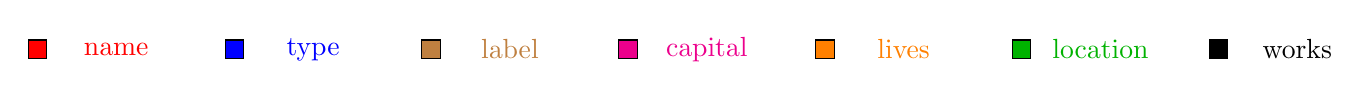
\begin{tikzpicture}[]
    \node[font=\bfseries,draw,fill=red] (nameColor) {};
    \node[red,right of = nameColor] (name) {name};

    \node[font=\bfseries,draw,fill=blue,right of = name,xshift=.5cm] (typeColor) {};
    \node[blue,right of = typeColor] (type) {type};

    \node[font=\bfseries,draw,fill=brown,right of = type,xshift=.5cm] (labelColor) {};
    \node[brown,right of = labelColor] (label) {label};

    \node[font=\bfseries,draw,fill=magenta,right of = label,xshift=.5cm] (capitalColor) {};
    \node[magenta,right of = capitalColor] (capital) {capital};

    \node[font=\bfseries,draw,fill=orange,right of = capital,xshift=.5cm] (livesColor) {};
    \node[orange,right of = livesColor] (lives) {lives};

    \node[font=\bfseries,draw,fill=black!30!green,right of = lives,xshift=.5cm] (locationColor) {};
    \node[black!30!green,right of = locationColor] (location) {location};

    \node[font=\bfseries,draw,fill=black,right of = location,xshift=.5cm] (worksColor) {};
    \node[black,right of = worksColor] (works) {works};
\end{tikzpicture}
%% vim: et:sw=4

    }
    \vspace{.25em}
    \begin{columns}[c]
        \column{.5\textwidth}
        \resizebox{\textwidth}{!}{
            \pgfplotstableread[header=false]{images/precision/error-graph-matrix.dat}{\graph} 
\pgfplotstablegetrowsof{images/precision/error-graph-matrix.dat}
\pgfmathsetmacro{\rows}{\pgfplotsretval}

%name = 1 = red
%type = 2 = blue
%label = 3 = brown
%capital = 4 = magenta
%lives = 5 = orange
%location = 6 = black!30!green
%works = 7 = black

\setbeamercovered{invisible}
\begin{tikzpicture}[draw=black, ultra thick]
    \uncover<1-1>{
        \foreach \col in {0,...,\rows} {%
            \foreach \row in {0,...,\rows} {%
                \ifthenelse{\row=0 \AND \col=0}{
                }
                {
                    \ifthenelse{\row=0}{
                        \node [Square] at ($(\col,-\row)-(0.5,0.5)$) {\col};
                    }
                    {
                        \ifthenelse{\col=0}{
                            \node [Square] at ($(\col,-\row)-(0.5,0.5)$) {\row};
                        }
                        {
                            \pgfmathsetmacro{\x}{int(\row-1)}
                            \pgfmathsetmacro{\y}{int(\col-1)}

                            \pgfplotstablegetelem{\x}{\y}\of{\graph} 

                            \begin{switch}{\pgfplotsretval}
                                \case{0}{
                                    \node [Square] at ($(\col,-\row)-(0.5,0.5)$) {};
                                }
                                \case{1}{
                                    \node [Red Square] at ($(\col,-\row)-(0.5,0.5)$) {};
                                }
                                \case{2}{
                                    \node [Blue Square] at ($(\col,-\row)-(0.5,0.5)$) {};
                                }
                                \case{3}{
                                    \node [Brown Square] at ($(\col,-\row)-(0.5,0.5)$) {};
                                }
                                \case{4}{
                                    \node [Magenta Square] at ($(\col,-\row)-(0.5,0.5)$) {};
                                }
                                \case{5}{
                                    \node [Orange Square] at ($(\col,-\row)-(0.5,0.5)$) {};
                                }
                                \case{6}{
                                    \node [Green Square] at ($(\col,-\row)-(0.5,0.5)$) {};
                                }
                                \case{7}{
                                    \node [Black Square] at ($(\col,-\row)-(0.5,0.5)$) {};
                                }
                                \case{8}{
                                    %% two colors: magenta and brown. Brown is drown with stripes below
                                    \node [Magenta Square] at ($(\col,-\row)-(0.5,0.5)$) {};
                                    \begin{scope}
                                        \clip (\col-1+.027,-\row-.027) rectangle (\col-.027,-\row-1+.027);
                                        \foreach \x in {0,0.4,...,\rows} {%
                                            \draw [brown,line width=4pt] (0,\x) -- (\rows,\x - \rows);
                                            \draw [brown,line width=4pt] (0,-\x) -- (\rows,-\x - \rows);
                                        }
                                    \end{scope}
                                }
                            \end{switch}
                        }
                    }
                }
            }
        }
    }

    \uncover<2-2>{
        \foreach \col in {0,...,\rows} {%
            \foreach \row in {0,...,\rows} {%
                \ifthenelse{\row=0 \AND \col=0}{
                }
                {
                    \ifthenelse{\row=0}{
                        \node [Square] at ($(\col,-\row)-(0.5,0.5)$) {\col};
                    }
                    {
                        \ifthenelse{\col=0}{
                            \node [Square] at ($(\col,-\row)-(0.5,0.5)$) {\row};
                        }
                        {
                            \pgfmathsetmacro{\x}{int(\row-1)}
                            \pgfmathsetmacro{\y}{int(\col-1)}

                            \pgfplotstablegetelem{\x}{\y}\of{\graph} 

                            \begin{switch}{\pgfplotsretval}
                                \case{0}{
                                    \node [Square] at ($(\col,-\row)-(0.5,0.5)$) {};
                                }
                                \case{1}{
                                    \node [Dim Red Square] at ($(\col,-\row)-(0.5,0.5)$) {};
                                }
                                \case{2}{
                                    \node [Dim Blue Square] at ($(\col,-\row)-(0.5,0.5)$) {};
                                }
                                \case{3}{
                                    \ifthenelse{\row=10 \AND \col=6}{
                                        \node [Brown Square] at ($(\col,-\row)-(0.5,0.5)$) {};
                                    }
                                    {
                                        \node [Dim Brown Square] at ($(\col,-\row)-(0.5,0.5)$) {};
                                    }
                                }
                                \case{4}{
                                    \node [Dim Magenta Square] at ($(\col,-\row)-(0.5,0.5)$) {};
                                }
                                \case{5}{
                                    \node [Dim Orange Square] at ($(\col,-\row)-(0.5,0.5)$) {};
                                }
                                \case{6}{
                                    \node [Dim Green Square] at ($(\col,-\row)-(0.5,0.5)$) {};
                                }
                                \case{7}{
                                    \node [Dim Black Square] at ($(\col,-\row)-(0.5,0.5)$) {};
                                }
                                \case{8}{
                                    %% two colors: magenta and brown. Brown is drown with stripes below
                                    \node [Dim Magenta Square] at ($(\col,-\row)-(0.5,0.5)$) {};
                                    \begin{scope}
                                        \clip (\col-1+.027,-\row-.027) rectangle (\col-.027,-\row-1+.027);
                                        \foreach \x in {0,0.4,...,\rows} {%
                                            \draw [brown!50,line width=4pt] (0,\x) -- (\rows,\x - \rows);
                                            \draw [brown!50,line width=4pt] (0,-\x) -- (\rows,-\x - \rows);
                                        }
                                    \end{scope}
                                }
                            \end{switch}
                        }
                    }
                }
            }
        }
        \draw [brown,ultra thick,line width=4pt] ($(6,-10)-(0.5,0.5)$) circle (1cm);
    }

    \uncover<3-3>{
        \foreach \col in {0,...,\rows} {%
            \foreach \row in {0,...,\rows} {%
                \ifthenelse{\row=0 \AND \col=0}{
                }
                {
                    \ifthenelse{\row=0}{
                        \node [Square] at ($(\col,-\row)-(0.5,0.5)$) {\col};
                    }
                    {
                        \ifthenelse{\col=0}{
                            \node [Square] at ($(\col,-\row)-(0.5,0.5)$) {\row};
                        }
                        {
                            \pgfmathsetmacro{\x}{int(\row-1)}
                            \pgfmathsetmacro{\y}{int(\col-1)}

                            \pgfplotstablegetelem{\x}{\y}\of{\graph} 

                            \begin{switch}{\pgfplotsretval}
                                \case{0}{
                                    \node [Square] at ($(\col,-\row)-(0.5,0.5)$) {};
                                }
                                \case{1}{
                                    \node [Dim Red Square] at ($(\col,-\row)-(0.5,0.5)$) {};
                                }
                                \case{2}{
                                    \node [Dim Blue Square] at ($(\col,-\row)-(0.5,0.5)$) {};
                                }
                                \case{3}{
                                    \node [Dim Brown Square] at ($(\col,-\row)-(0.5,0.5)$) {};
                                }
                                \case{4}{
                                    \node [Dim Magenta Square] at ($(\col,-\row)-(0.5,0.5)$) {};
                                }
                                \case{5}{
                                    \node [Dim Orange Square] at ($(\col,-\row)-(0.5,0.5)$) {};
                                }
                                \case{6}{
                                    \ifthenelse{\row=8 \AND \col=10}{
                                        \node [Green Square] at ($(\col,-\row)-(0.5,0.5)$) {};
                                    }
                                    {
                                        \node [Dim Green Square] at ($(\col,-\row)-(0.5,0.5)$) {};
                                    }
                                }
                                \case{7}{
                                    \node [Dim Black Square] at ($(\col,-\row)-(0.5,0.5)$) {};
                                }
                                \case{8}{
                                    %% two colors: magenta and brown. Brown is drown with stripes below
                                    \node [Dim Magenta Square] at ($(\col,-\row)-(0.5,0.5)$) {};
                                    \begin{scope}
                                        \clip (\col-1+.027,-\row-.027) rectangle (\col-.027,-\row-1+.027);
                                        \foreach \x in {0,0.4,...,\rows} {%
                                            \draw [brown!50,line width=4pt] (0,\x) -- (\rows,\x - \rows);
                                            \draw [brown!50,line width=4pt] (0,-\x) -- (\rows,-\x - \rows);
                                        }
                                    \end{scope}
                                }
                            \end{switch}
                        }
                    }
                }
            }
        }
        \draw [black!30!green,ultra thick,line width=4pt] ($(10,-8)-(0.5,0.5)$) circle (1cm);
    }
\end{tikzpicture}
\setbeamercovered{transparent}
%% vim: et:sw=4

        }

        \column{.5\textwidth}
        \resizebox{\textwidth}{!}{
            \input{images/precision/error-graph}
        }
    \end{columns}
}

\frame{
    \frametitle{Summary Precision}
    \begin{block}{Errors Classification}
        \begin{itemize}
            \item Type
            \item Attribute
            \item Connectivity
        \end{itemize}
    \end{block}
    \begin{block}{Precision Measure}
        \begin{itemize}
            \item Based on the set of \textbf{true} (TP) and \textbf{false} (FP) positives edges:
                \begin{equation*}
                    Prec(R, x) = \frac{\vert TP(x) \vert}{\vert TP(x) \bigcup FP(R, x) \vert}
                \end{equation*}
        \end{itemize} 
    \end{block}
}

\subsection{Evaluation}

\frame[shrink]{
    \frametitle{Evaluation Dimensions}
    \vspace{2em}
    \Wider{
        \uncover<2->{
            \begin{block}{How small the summary is compared to the original graph ?}
                Ratio of order and size of the graph $G$ to the summary $\mathcal{S}$:

                $$
                G:\mathcal{S} = \frac{\vert V \vert + \vert A \vert}{\vert \mathcal{W} \vert + \vert \mathcal{B} \vert}
                $$
            \end{block}
        }
        \uncover<3->{
            \begin{block}{How performant and scalable is the summarization process ?}
                Record of the time spent on the process
            \end{block}
        }
        \uncover<4->{
            \begin{block}{How precise is the generated summary ?}
                Average precision of the summary:

                $$
                \frac{1}{\vert \mathcal{W}_{fbt} \vert} \times \sum_{c \in \mathcal{W}}{\frac{1}{\vert C(c) \vert} \times \sum_{x \in C(c)}{Prec(R, x)}}
                $$
            \end{block}
        }
    }
    \setbeamercovered{invisible}
    \begin{tikzpicture}[remember picture]
        %\draw[step=1cm,gray,ultra thick,overlay] (0,0) grid (12,12);
        %\draw[step=.1cm,blue,overlay] (0,0) grid (12,12);

        \uncover<5-5>{
            \draw[red,thick,overlay] (6.9,.7) rectangle (8.8,1.3);
        }
        \uncover<6-6>{
            \draw[red,thick,overlay] (4.4,.2) rectangle (8.8,1.5);
        }
        \uncover<7-7>{
            \draw[red,thick,overlay] (2.1,.2) rectangle (8.8,1.5);
        }
    \end{tikzpicture}
    \setbeamercovered{transparent}
}

\frame{
    \frametitle{Datasets}
    \vspace{.3cm}
    \begin{columns}[c]
        \column{.5\textwidth}
        \setbeamercovered{invisible}
\begin{figure}
    \centering
    \resizebox{!}{.8\textheight}{
        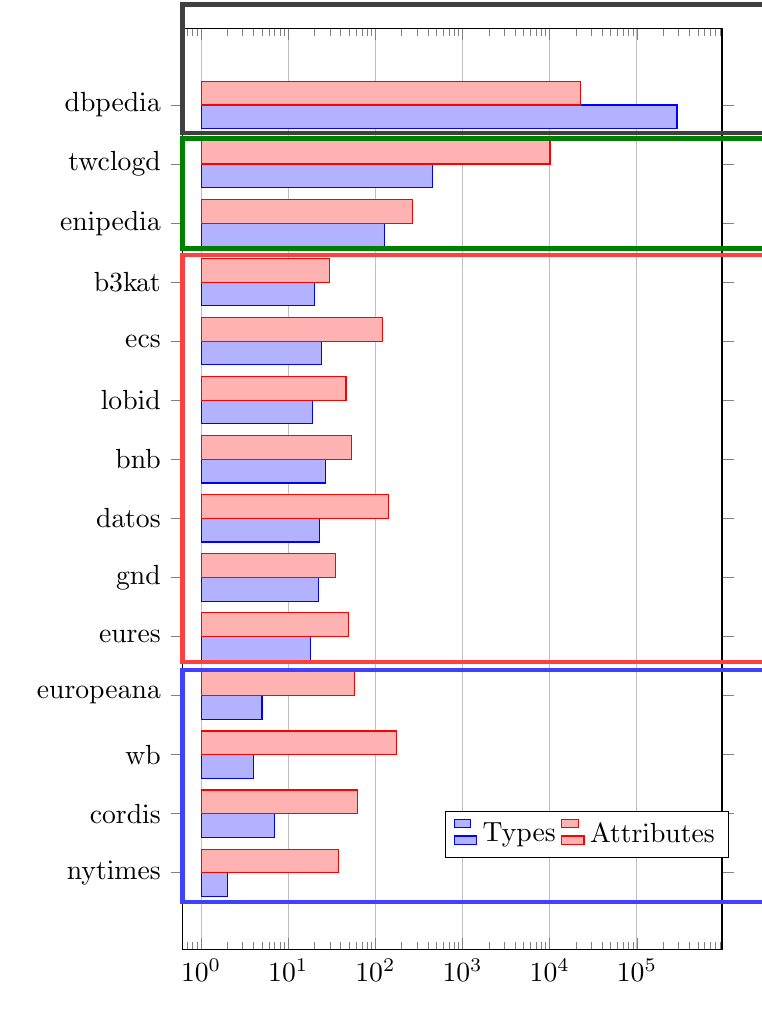
\begin{tikzpicture}[remember picture]
            \begin{axis}[
                    xbar=0pt,
                    y=.75cm,
                    symbolic y coords={nytimes,cordis,wb,europeana,eures,gnd,datos,bnb,lobid,ecs,b3kat,enipedia,twclogd,dbpedia},
                    bar width=0.3cm,
                    ytick=data,
                    xmode = log,
                    xmajorgrids = true,
                    legend style={at={(0.75,0.15)}, anchor=north,legend columns=-1},
                ]
                \addplot coordinates { (2,nytimes) (7,cordis) (4,wb) (5,europeana) (18,eures) (22,gnd) (23,datos) (27,bnb) (19,lobid) (24,ecs) (20,b3kat) (128,enipedia) (450,twclogd) (288524,dbpedia) };
                \addplot coordinates { (38,nytimes) (63,cordis) (174,wb) (58,europeana) (49,eures) (35,gnd) (143,datos) (53,bnb) (46,lobid) (120,ecs) (30,b3kat) (267,enipedia) (10060,twclogd) (22369,dbpedia) };
                \legend{Types,Attributes}
            \end{axis}

            \uncover<2->{
                % very high
                \draw[black!75,ultra thick,overlay] (0,12) rectangle (17.2,10.37) node[midway] {\textbf{\textcolor{black}{Very High}}};
            }

            \uncover<3->{
                % high
                \draw[black!50!green,ultra thick,overlay] (0,10.3) rectangle (17.2,8.9) node[midway] {\textbf{\textcolor{black!50!green}{High}}};
            }

            \uncover<4->{
                % medium
                \draw[red!75,ultra thick,overlay] (0,8.82) rectangle (17.2,3.65) node[midway] {\textbf{\textcolor{red}{Medium}}};
            }

            \uncover<5->{
                % low
                \draw[blue!75,ultra thick,overlay] (0,3.55) rectangle (17.2,0.6) node[midway] {\textbf{\textcolor{blue}{Low}}};
            }
        \end{tikzpicture}
    }
\end{figure}
\setbeamercovered{transparent}
%% vim: et:sw=4


        \column{.5\textwidth}
        \setbeamercovered{invisible}
\begin{figure}
    \centering
    \resizebox{!}{.8\textheight}{
        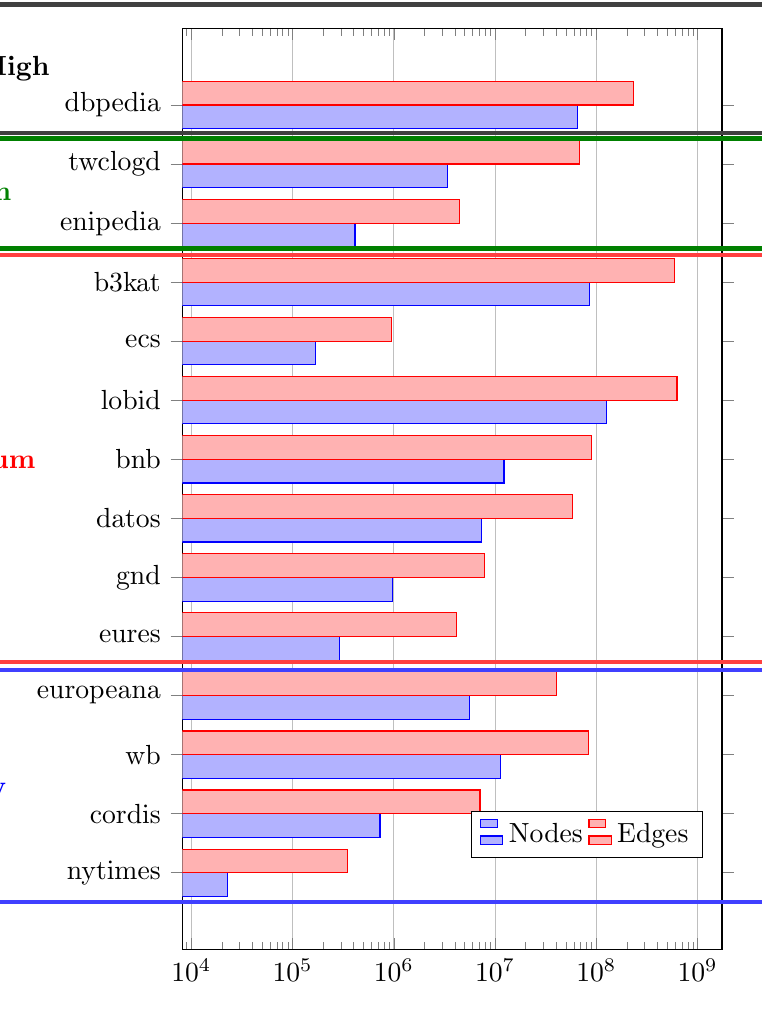
\begin{tikzpicture}
            \begin{axis}[
                    xbar=0pt,
                    y=.75cm,
                    symbolic y coords={nytimes,cordis,wb,europeana,eures,gnd,datos,bnb,lobid,ecs,b3kat,enipedia,twclogd,dbpedia},
                    bar width=0.3cm,
                    ytick=data,
                    xmode = log,
                    xmajorgrids = true,
                    legend style={at={(0.75,0.15)}, anchor=north,legend columns=-1},
                ]
                \addplot coordinates { (22662,nytimes) (729780,cordis) (11210832,wb) (5559452,europeana) (288862,eures) (962930,gnd) (7412312,datos) (12246306,bnb) (124691274,lobid) (167390,ecs) (85795956,b3kat) (413520,enipedia) (3398947,twclogd) (65042837,dbpedia) };
                \addplot coordinates { (345888,nytimes) (7101623,cordis) (84345613,wb) (40773834,europeana) (4146421,eures) (7940373,gnd) (58048932,datos) (89733453,bnb) (625941644,lobid) (955112,ecs) (592778746,b3kat) (4463566,enipedia) (67505792,twclogd) (233051608,dbpedia) };
                \legend{Nodes,Edges}
            \end{axis}

            \uncover<2->{
                %\draw[step=1cm,gray,ultra thick,overlay] (-20,-2) grid (20,12);
                %\draw[step=.1cm,blue,overlay] (-20,-2) grid (20,12);
                % very high
                \draw[black!75,ultra thick,overlay] (-13,12) rectangle (7.8,10.37) node[midway] {\textbf{\textcolor{black}{Very High}}};
                % high
                \draw[black!50!green,ultra thick,overlay] (-13,10.3) rectangle (7.8,8.9) node[midway] {\textbf{\textcolor{black!50!green}{High}}};
                % medium
                \draw[red!75,ultra thick,overlay] (-13,8.82) rectangle (7.8,3.65) node[midway] {\textbf{\textcolor{red}{Medium}}};
                % low
                \draw[blue!75,ultra thick,overlay] (-13,3.55) rectangle (7.8,0.6) node[midway] {\textbf{\textcolor{blue}{Low}}};
            }
        \end{tikzpicture}
    }
\end{figure}
\setbeamercovered{transparent}
%% vim: et:sw=4

    \end{columns}
}

\setbeamercovered{invisible}
\frame{
    \frametitle{Tradeoffs: Precision VS. Compression}
    \begin{figure}
        \centering
        \begin{subfigure}[t]{0.46\textwidth}
            \resizebox{\textwidth}{!}{
                \begin{tikzpicture}
    \begin{axis}[
            scatter/classes={
                a={mark=square},%
                b={mark=star},%
                c={mark=oplus},%
                d={mark=o},%
                e={mark=triangle},%
                f={mark=pentagon}
            },
            ylabel=$Connectivity$,
            xlabel=$Compression \; Ratio$,
            mark options={scale=2},
            legend style={at={(.95,0.9)}}
        ]
        \addplot[scatter,only marks,scatter src=explicit symbolic]
            coordinates {
                (247305.94, 0.14856667) [a]
                (150252.41, 0.2356) [b]
                (1433.53, 0.2736) [c]
                (1314.50, 0.4238) [d]
                (1268.24, 0.51803333) [e]
                (1184.26, 0.64733333) [f]
            };
        \legend{$R_{ut}$, $R_{t}$, $R_{a}$, $R_{at}$, $R_{ioa}$, $R_{ioat}$}
    \end{axis}
    \uncover<2->{
        \draw[red,ultra thick] (.2,5.5) rectangle (1,1.2);
        \draw[blue,ultra thick] (3.6,1.7) rectangle (6.6,.2);
    }
    \uncover<3-4>{
        \draw[draw=none,pattern=north west lines,pattern color=red,ultra thick] (.2,2.1) rectangle (1,1.2);
        \draw[draw=none,pattern=north east lines,pattern color=blue,ultra thick] (3.6,1.7) rectangle (4.6,1);
    }
    \uncover<4-4>{
        \draw[draw=none,pattern=north west lines,pattern color=red,ultra thick] (.2,3.5) rectangle (1,2.8);
        \draw[draw=none,pattern=north east lines,pattern color=blue,ultra thick] (.2,3.5) rectangle (1,2.8);
    }
    \uncover<5-5>{
        \draw[draw=none,pattern=dots,pattern color=black!50!green,ultra thick] (.2,5.5) rectangle (1,3.7);
    }
\end{tikzpicture}
%% vim: et:sw=4

            }
            \caption{Connectivity precision versus compression ratio.}
        \end{subfigure}
        \quad
        \begin{subfigure}[t]{0.46\textwidth}
            \resizebox{\textwidth}{!}{
                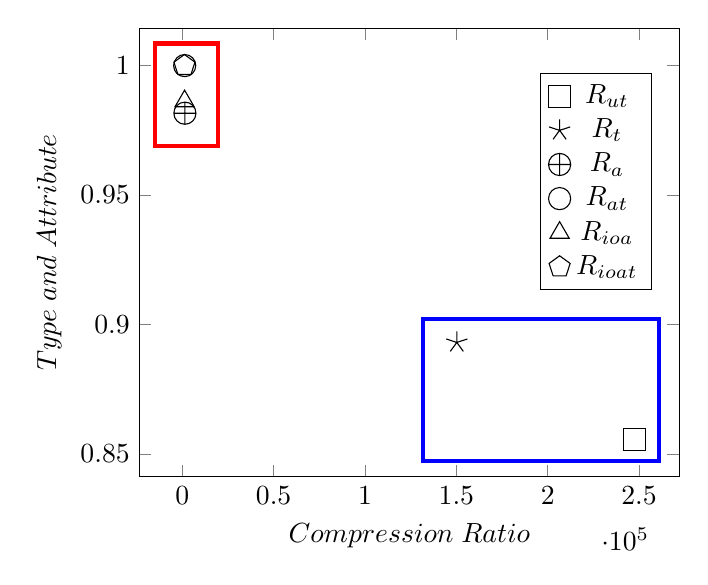
\begin{tikzpicture}
    \begin{axis}[
            scatter/classes={
                a={mark=square},%
                b={mark=star},%
                c={mark=oplus},%
                d={mark=o},%
                e={mark=triangle},%
                f={mark=pentagon}
            },
            ylabel=$Type \; and \; Attribute$,
            xlabel=$Compression \; Ratio$,
            mark options={scale=2},
            legend style={at={(0.95,0.9)}}
        ]
        \addplot[scatter,only marks,scatter src=explicit symbolic]
            coordinates {
                (247305.94, 0.85565) [a]
                (150252.41, 0.89303333) [b]
                (1433.53, 0.9816) [c]
                (1314.50, 1.0000) [d]
                (1268.24, 0.98623333) [e]
                (1184.26, 1.0000) [f]
            };
        \legend{$R_{ut}$, $R_{t}$, $R_{a}$, $R_{at}$, $R_{ioa}$, $R_{ioat}$}
    \end{axis}
    \uncover<2->{
        \draw[red,ultra thick] (.2,5.5) rectangle (1,4.2);
        \draw[blue,ultra thick] (3.6,2) rectangle (6.6,.2);
    }
\end{tikzpicture}
%% vim: et:sw=4

            }
            \caption{Type and attribute precision versus compression ratio.}
        \end{subfigure}
    \end{figure}
}

\frame{
    \frametitle{Tradeoffs: Precision VS. Performance}
    \begin{figure}
        \centering
        \begin{subfigure}[t]{0.46\textwidth}
            \resizebox{\textwidth}{!}{
                \begin{tikzpicture}
    \begin{axis}[
        grid=both,
        scatter/classes={
            a={mark=square},%
            b={mark=star},%
            c={mark=oplus},%
            d={mark=o},%
            e={mark=triangle},%
            f={mark=pentagon}
        },
        ylabel=$Connectivity$,
        xlabel=$CPU \; (ms)$,
        mark options={scale=2},
        legend style={at={(0.25,0.9)}}
    ]
    \addplot[scatter,only marks,scatter src=explicit symbolic]
        coordinates {
            (20384066, 0.14856667) [a]
            (17949001, 0.2356) [b]
            (20892062, 0.2736) [c]
            (20885921, 0.4238) [d]
            (20934061, 0.51803333) [e]
            (20561815, 0.64733333) [f]
        };
        \legend{$R_{ut}$, $R_{t}$, $R_{a}$, $R_{at}$,
        $R_{ioa}$, $R_{ioat}$}
    \end{axis}
    \uncover<2->{
        \draw[red,ultra thick] (5.2,5.5) rectangle (6.6,1.2);
        \draw[blue,ultra thick] (.2,1.7) rectangle (5.6,.2);
    }
    \uncover<3-3>{
        \draw[draw=none,pattern=north west lines,pattern color=red,ultra thick] (5.2,5.5) rectangle (6,4.8);
    }
    \uncover<4-4>{
        \draw[draw=none,pattern=north east lines,pattern color=blue,ultra thick] (.2,1.7) rectangle (1,1);
    }
\end{tikzpicture}

            }
            \caption{Connectivity precision versus summarisation performance.}
        \end{subfigure}
        \quad%
        \begin{subfigure}[t]{0.46\textwidth}
            \resizebox{\textwidth}{!}{
                \begin{tikzpicture}
    \begin{axis}[
        scatter/classes={
            a={mark=square},%
            b={mark=star},%
            c={mark=oplus},%
            d={mark=o},%
            e={mark=triangle},%
            f={mark=pentagon}
        },
        ylabel=$Type \; and \; Attribute$,
        xlabel=$CPU \; (ms)$,
        mark options={scale=2},
        legend style={at={(0.25,0.9)}}
    ]
    \addplot[scatter,only marks,scatter src=explicit symbolic]
        coordinates {
            (20384066, 0.85565) [a]
            (17949001, 0.89303333) [b]
            (20892062, 0.9816) [c]
            (20885921, 1) [d]
            (20934061, 0.98623333) [e]
            (20561815, 1) [f]
        };
        \legend{$R_{ut}$, $R_{t}$, $R_{a}$, $R_{at}$, $R_{ioa}$, $R_{ioat}$}
    \end{axis}
    \uncover<2->{
        \draw[red,ultra thick] (5.2,5.6) rectangle (6.6,4.2);
        \draw[blue,ultra thick] (.2,2) rectangle (5.6,.2);
    }
    \uncover<3-3>{
        \draw[draw=none,pattern=north west lines,pattern color=red,ultra thick] (5.2,5.6) rectangle (6,4.8);
    }
    \uncover<4-4>{
        \draw[draw=none,pattern=north east lines,pattern color=blue,ultra thick] (.2,2) rectangle (1,1.4);
    }
\end{tikzpicture}

            }
            \caption{Type and attribute precision versus summarisation performance.}
        \end{subfigure}
    \end{figure}
}
\setbeamercovered{transparent}
%% vim: et:sw=4
